\documentclass{ximera}

\input{../preamble}
\author{Ivo Terek and Elizabeth Campolongo}
\license{Creative Commons Attribution-ShareAlike 4.0 International License}
\acknowledgement{}

\title{Slopes of Secant Lines as a Function of h}

\begin{document}
\begin{abstract}
  
\end{abstract}
\maketitle


%\typeout{************************************************}
%\typeout{Motivating Questions}
%\typeout{************************************************}

\begin{motivatingQuestions}\begin{itemize}
\item How can we rewrite the average rate of change of a function in terms of the horizontal distance, h, between the points?  Why would we want to do that?
\item What are some algebra techniques that allow us to simplify the average rate of change for an arbitrary h?
\item What does it tell us when we put in small values for h?
\end{itemize}\end{motivatingQuestions}


%\typeout{************************************************}
%\typeout{Subsection Introduction}
%\typeout{************************************************}

\section{Introduction}

We have discussed a secant line to the graph of a function $y=f(x)$ from $(a,f(a))$ to $(b,f(b))$, and the fact that the slope, $m$, of this line is the average rate of change of the function $f$ on the interval $[a,b]$, $\av_{[a,b]}$. Furthermore, recall that we can let $h=b-a$, so that the slope expression becomes 
%
$$m=\frac{f(a+h)-f(a)}{h},$$
where $h$ is the horizontal distance between the points.

\begin{image}[2in]
		  \begin{tikzpicture}
		  \draw [thick, scale = 3, domain = -.5:2, smooth, variable =\x] plot ({\x},  {3/4*exp(\x)*cos(deg(\x)) + 1/2*exp(\x)*sin(deg(\x))});%{\x*(3-2*\x*\x)});
		    \coordinate (C) at (0,2.8);
		    \coordinate (D) at (5,1);
		    \coordinate (E) at (5,7.5);
		   % \draw[decoration={brace,mirror,raise=.2cm},decorate,thin] (0,2)--(4,2);
		   % \draw[decoration={brace,mirror,raise=.2cm},decorate,thin] (4,2)--(4,6.5);
		  %  \draw[decoration={brace,raise=.2cm},decorate,thin] (0,2)--(4,6.5);
		    \draw[blue] (C)--(E)--cycle;
		 %   \draw[dotted] (C) edge (D);
		%    \draw[dotted] (E) edge (D);
		      \node at (2,7) {$y= f(x)$};
		   \node at (.4,4) {$(a, f(a))$};
		   % \node[rotate=-90] at (4+.5,4) {A'};
		 %   \node[rotate=35] at (.8,4.8) {$f(x)-f(x_1) = m(x-x_1)$};
		    \node at (5.1,7.8) {$(a+h,f(a+h))$};
		%    \node at (-4.7, 1) {$(x_1,y_1)$};
		  \end{tikzpicture}
		\end{image}

One of the main objectives of Calculus is to understand instantaneous rates of change, as opposed to average rates of change. Namely, what is the behavior of the expression 
$$\frac{f(a+h)-f(a)}{h}$$
when $h$ gets very small? Geometrically, making $h$ become very small is making the secant line through $(a,f(a))$ and $(a+h,f(a+h))$ approach a certain line --- the tangent line to the graph of $y=f(x)$ at the point $a$. This is demonstrated in the figure below, where the secant line is blue, and the line tangent to the graph at $a$ is in red. 

\begin{image}[2.5in]
		  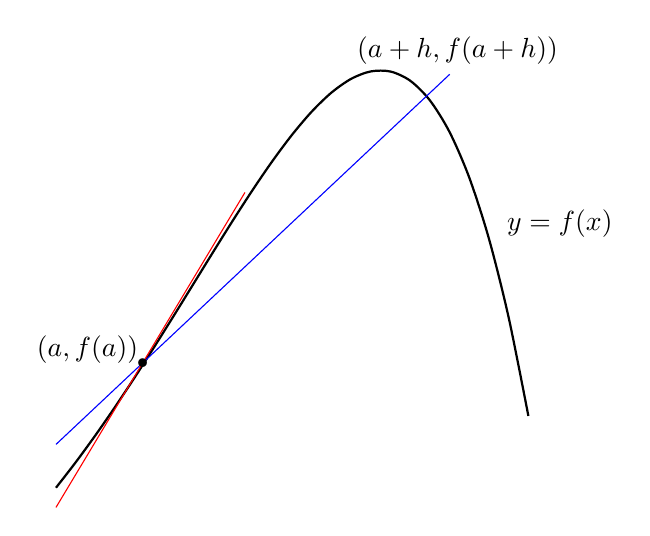
\begin{tikzpicture}
		  \draw [thick, scale = 3, domain = -0:2, smooth, variable =\x] plot ({\x},  {3/4*exp(\x)*cos(deg(\x)) + 1/2*exp(\x)*sin(deg(\x))});%{\x*(3-2*\x*\x)});
		    \coordinate (C) at (0,2.8);
		    \coordinate (D) at (5,1);
		    \coordinate (E) at (5,7.5);
		    \coordinate (A) at (0,2);
		    \coordinate (B) at (2.4,6);
		   % \draw[decoration={brace,mirror,raise=.2cm},decorate,thin] (0,2)--(4,2);
		   % \draw[decoration={brace,mirror,raise=.2cm},decorate,thin] (4,2)--(4,6.5);
		  %  \draw[decoration={brace,raise=.2cm},decorate,thin] (0,2)--(4,6.5);
		    \draw[blue] (C)--(E)--cycle;
		    \draw[red] (A)--(B)--cycle;
		 %   \draw[dotted] (C) edge (D);
		%    \draw[dotted] (E) edge (D);
		      \node at (6.4,5.6) {$y= f(x)$};
		   \node at (.4,4) {$(a, f(a))$};
		   % \node[rotate=-90] at (4+.5,4) {A'};
		 %   \node[rotate=35] at (.8,4.8) {$f(x)-f(x_1) = m(x-x_1)$};
		    \node at (5.1,7.8) {$(a+h,f(a+h))$};
		%    \node at (-4.7, 1) {$(x_1,y_1)$};
		\node[black, scale = 3] at (intersection of C--E and A--B){.};
		  \end{tikzpicture}
		\end{image}

Follow the link below to an example Desmos graph where you can see the effect of changing the value of $h$ on the secant line in real-time.
\desmos{f6fh2wkrrn}{800}{600}

%tangent line parallel to secant line
%\begin{image}[2in]
%		  \begin{tikzpicture}
%		  \draw [thick, scale = 3, domain = -.5:2, smooth, variable =\x] plot ({\x},  {3/4*exp(\x)*cos(deg(\x)) + 1/2*exp(\x)*sin(deg(\x))});%{\x*(3-2*\x*\x)});
%		    \coordinate (C) at (0,2.8);
%		    \coordinate (D) at (5,1);
%		    \coordinate (E) at (5,7.5);
%		    \coordinate (A) at (1.5,5.41);
%		    \coordinate (B) at (4.5,8.23);
%		   % \draw[decoration={brace,mirror,raise=.2cm},decorate,thin] (0,2)--(4,2);
%		   % \draw[decoration={brace,mirror,raise=.2cm},decorate,thin] (4,2)--(4,6.5);
%		  %  \draw[decoration={brace,raise=.2cm},decorate,thin] (0,2)--(4,6.5);
%		    \draw[blue] (C)--(E)--cycle;
%		    \draw[red] (A)--(B)--cycle;
%		 %   \draw[dotted] (C) edge (D);
%		%    \draw[dotted] (E) edge (D);
%		      \node at (6.4,5.6) {$y= f(x)$};
%		   \node at (.4,4) {$(a, f(a))$};
%		   % \node[rotate=-90] at (4+.5,4) {A'};
%		 %   \node[rotate=35] at (.8,4.8) {$f(x)-f(x_1) = m(x-x_1)$};
%		    \node at (5.1,7.8) {$(a+h,f(a+h))$};
%		%    \node at (-4.7, 1) {$(x_1,y_1)$};
%		  \end{tikzpicture}
%		\end{image}


The slope of such a tangent line, when it exists, is called the derivative of $f$ at $a$. Here, we'll discuss difference quotients and several examples, to prepare you to learn those things in more detail in a future Calculus class.


\section{Definitions and examples}

\begin{callout}
  {\bf Definition:} The difference quotient of a function $y=f(x)$ at a point $a$ of its domain is the quantity $$\frac{f(a+h)-f(a)}{h},$$i.e., the average rate of change of $f$ on the interval $[a,a+h]$.
\end{callout}

\begin{example}
  Find the difference quotients of the following functions, at the given point. 
  \begin{enumerate}[label=\alph*.]
  \item $f(x)=x^2$, $a=2$.

    \begin{explanation}
      Let's evaluate it directly:
      \begin{align*}
        \frac{f(2+h)-f(2)}{h} &= \frac{(2+h)^2-2^2}{h} = \frac{2^2+4h+h^2-2^2}{h} \\ &= \frac{4h+h^2}{h} = h+4.
      \end{align*}
      We thus have an equation for the slope of the secant line from $(2,f(2))$ to $(2+h,f(2+h))$: 
      $$\av_{[2,2+h]}= m = h+4.$$
      Recall from Example 1(a) of Section 12-3-1, that we calculated the slope of the secant line from $(1,f(1))$ to $(2,f(2))$. Letting $h=-1$, we see that this gives the same answer for the slope of that secant line.
      
      Furthermore, if we now let $h \rightarrow 0$, this expression, $\frac{f(2+h)-f(2)}{h} \rightarrow 4$.
    \end{explanation}
    
  \item $f(x) = \sin (x), \ a =\frac{\pi}{3}$.\\
  \begin{explanation}
  Again, we evaluate directly:
  \begin{equation*}
   \frac{f(\frac{\pi}{3} + h) - f(\frac{\pi}{3})}{h} = \frac{\sin(\frac{\pi}{3} +h) - \sin (\frac{\pi}{3})}{h}
  \end{equation*}
  Recognizing that we cannot further simplify this expression in its current form, we replace $\sin((\pi/3) +h)$ using the sine sum expression:
  \begin{align*}
  \frac{\sin(\frac{\pi}{3} +h) - \sin (\frac{\pi}{3})}{h} 
  &= \frac{\sin(\frac{\pi}{3})\cos (h) + \cos(\frac{\pi}{3}) \sin( h) - \frac{\sqrt{3}}{2}}{h} \\
  &= \frac{1}{2h}\big(\sqrt{3}(\cos (h) -1) + \sin( h)\big)
  \end{align*}
  This gives a less easy to visualize equation for the slope of the secant line from $(a,f(a))$ to $(a+h,f(a+h))$, for $a=\frac{\pi}{3}$: 
  %
  $$\av_{[\frac{\pi}{3},\frac{\pi}{3}+h]}= m =\frac{1}{2h}\big(\sqrt{3}(\cos (h) -1) + \sin( h)\big).$$ 
  %
  However, consider $h=\frac{\pi}{2}$, so that we are looking at the secant line from $(\pi/3, f(\pi/3))$ to $(5\pi/6, f(5\pi/6))$. We then see that 
  %
  $$ \frac{f(\frac{\pi}{3} + h) - f(\frac{\pi}{3})}{h} = \frac{1}{2} \cdot \frac{\pi}{2}\big(\sqrt{3}(\cos\Big(\frac{\pi}{2}\Big) -1)+ \sin\Big(\frac{\pi}{2}\Big) \big)= 0,$$
 as before.
 
 Furthermore, what happens as we let $h \rightarrow 0$. Consider $h =\frac{\pi}{6}$, then we have 
  \begin{align*}
   \frac{f(\frac{\pi}{3} + h) - f(\frac{\pi}{3})}{h} &= \frac{1}{2} \cdot \frac{6}{\pi}\big(\sqrt{3}(\cos\Big(\frac{\pi}{6}\Big) -1) + \sin\Big(\frac{\pi}{6}\Big)\big)\\
   &= \frac{3}{\pi}\Big(\sqrt{3}\Big(\frac{\sqrt{3}}{2} -1\Big)+ \frac{1}{2}\Big)\\
   &=\frac{6-3\sqrt{3}}{\pi},
   \end{align*}
   Note that this is greater than 0. Think about the graph of $y=sin(x)$. It is increasing on the interval $\big[\frac{\pi}{3}, \frac{\pi}{2}\big]$.
   
   Follow the Desmos link to explore more initial values of $x$ and see what happens as you adjust $h$ smaller and smaller to zero.
   \desmos{xbi081bx3w}{800}{600}

    \end{explanation}
  
  \item $f(x) = 2x+3, \ a = -1$.\\
  \begin{explanation}
  Evaluate directly:
  \begin{equation*}
  \frac{f(-1 + h) - f(-1)}{h} = \frac{2(h-1) + 3 - (2(-1)+3)}{h} = \frac{2h-2 +2}{h} = 2 
  \end{equation*}
  %
  Observe that the equation for the slope of the secant line from $(-1,f(-1))$ to $(-1+h,f(-1+h))$ is simply
  $$\av_{[-1,-1+h]}=  m = 2.$$
  
 Recall from Example 1(c) of Section 12-3-1, that the equation of the secant line from $(-1,f(-1))$ to $(3,f(3))$ was simply $f(x)$. Why was this?
  
Now, this tells us that regardless of the points we choose, the secant line between them will have the same slope and equation as the line itself.
  \end{explanation}
   \end{enumerate}
\end{example}


\end{document}
